\documentclass{article}

\usepackage[utf8]{inputenc}
\usepackage{setspace}
\usepackage{geometry}
\usepackage{graphicx}
\usepackage{caption}
\usepackage{indentfirst}
\usepackage{anyfontsize}
\usepackage{textcomp}
\usepackage{float}

\graphicspath{}



\title{Discrete Population Modeling}
\author{Geneva Porter}
\date{20 September 2018}

\begin{document}
	
\begin{titlepage}
\maketitle
\thispagestyle{empty}



\centering
\large \it San Diego State University

Professor Mahaffy, Math 636
\end{titlepage}

\section*{Problem 1: Italy and Growth Rates}

In this problem, we examine the growth rate of Italy and the resulting effect on their population. In Figures 1 and 2, two different population models are depicted. The first displays the projection of Italy's population with a constant growth rate of 6.1\%. This growth rate was calculated by determining the average of the growth rates between 1960 \& 1970, and 1970 \& 1980. We can see that while this model correctly predicts the population for 1970 and 1980, it becomes uselessly inaccurate for 1980 and 1990. 

A more useful model is one that takes into account Italy's declining growth rate. The dashed line in Figure 2 considers that while births may increase the population by about 7\% each year, deaths and other factors reduce this growth by about 1.8\% per year, cumulatively. This model is significantly more accurate for predicting the population for 1990 and 2000, and would suggest that Italy's population would begin to decline between 2000 and 2010. 

As with any model, predictions could be improved with more data. We might find that with earlier years, Italy's population grew significantly faster, and the cumulative decline was significantly higher as well. This might give the linear model of growth rate a greater intercept value but a slope with a steeper negative value. A model with these modifications may more accurately predict a more severely declining growth rate as seen by the empirical data. Another way this model can be improved is by an analysis of the methods of collection for population. Various differing methods over the decades may have given inaccurate data, thus providing less accurate models.

\vspace{5mm}

\begin{figure}[H]
\centering{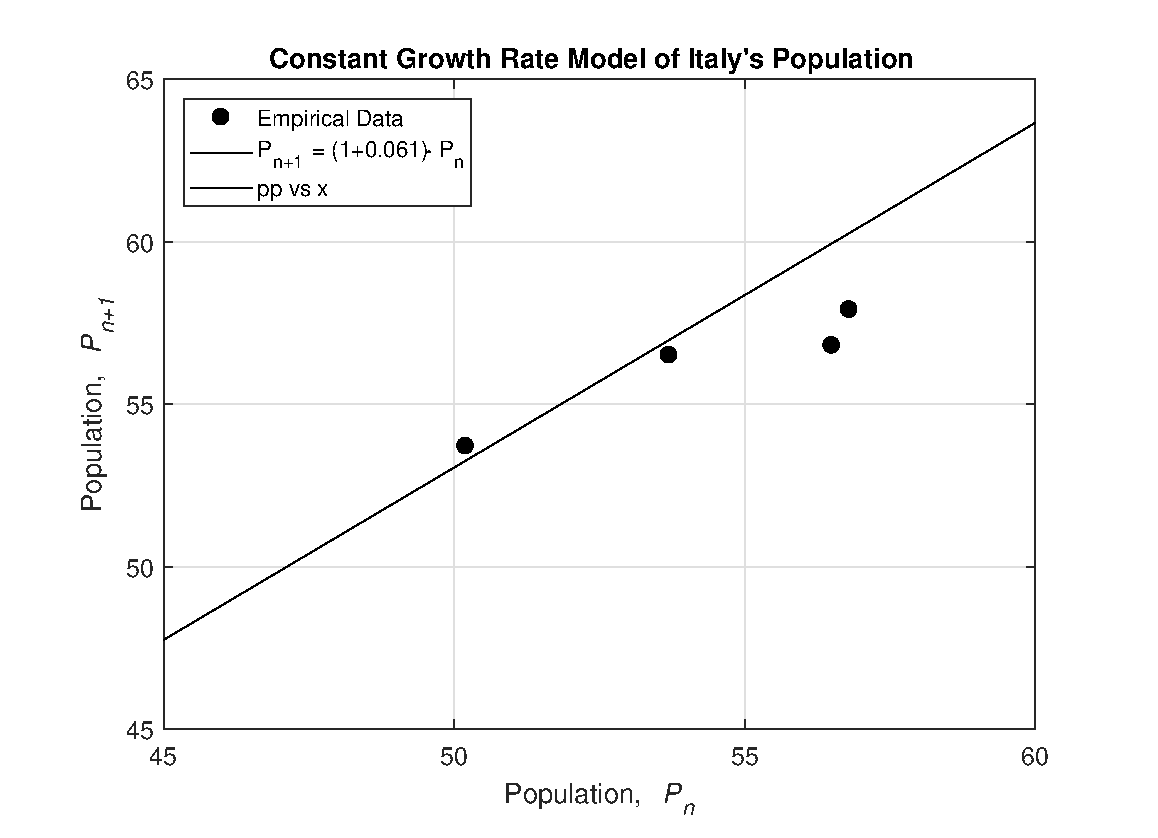
\includegraphics[width=12cm]{problem1.eps}}
	\caption{$P_{n+1}$ vs. $P_n$}
\end{figure}

\vspace{5mm}

\begin{figure}[H]
	\centering{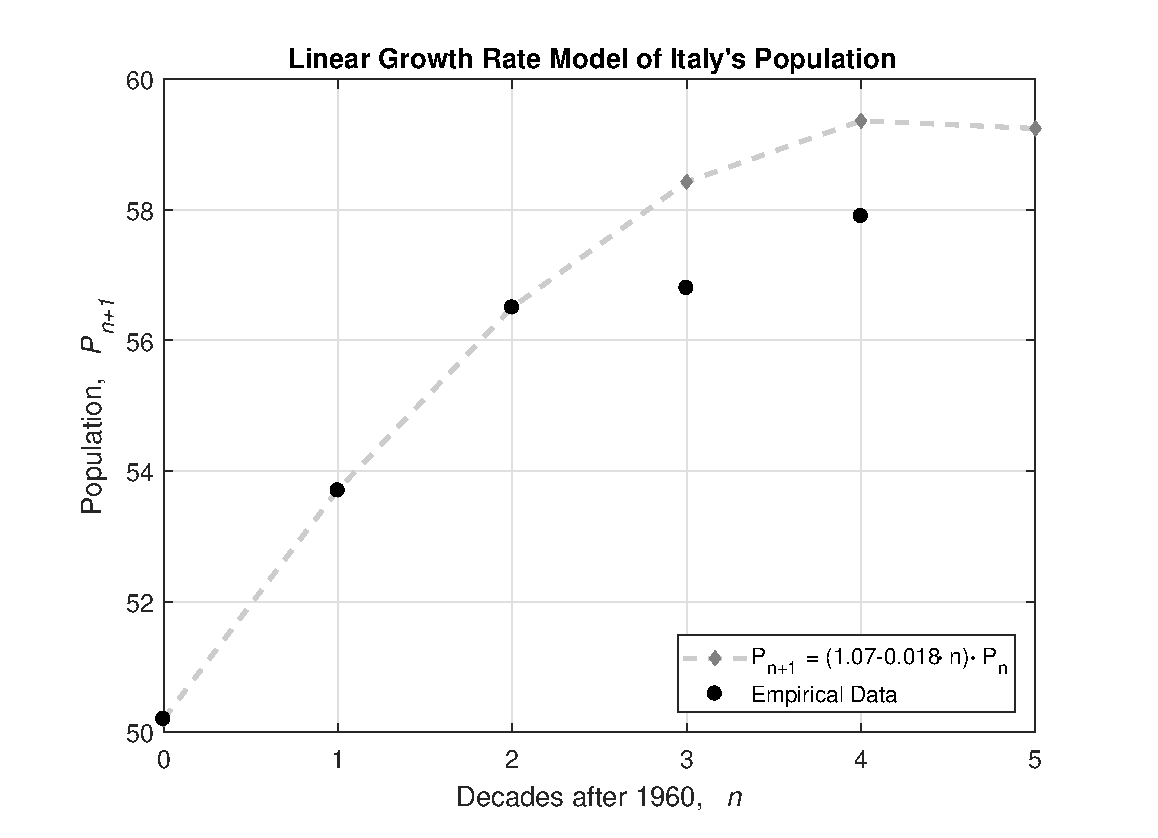
\includegraphics[width=12cm]{problem1b.eps}}
	\caption{$P$ vs. $n$}
\end{figure}

\vspace{5mm}


\section*{Problem 2: Island Moth Populations}

Here we examine a species of moth that lives on an island with a continually growing population. We have a constant growth rate of 85\% in addition to an extra 500 moths that immigrate each year.

Figure 3 displays the updating growth function, a solid line, alongside the identity line, the dashed line. we can see that there is an intersection point at around 3330. If our starting population were at or below this number, the species would likely reach and then remain at this constant population. However, our starting population is at 7000. Therefore the moths' population will continue to grow infinitely, or until they run out of resources, whichever comes first. At this point the population would likely see a dramatic decline, and perhaps reach the stable equilibrium soon after.

Clearly, the model of a constant growth rate is unrealistic. To more accurately model the population, we would need a changing growth rate. Taking into account availability of recourses and seasonal disturbances, it is likely that a dynamic growth would show a declining growth rate to account for crowding effects.

\vspace{5mm}

\begin{figure}[H]
	\centering{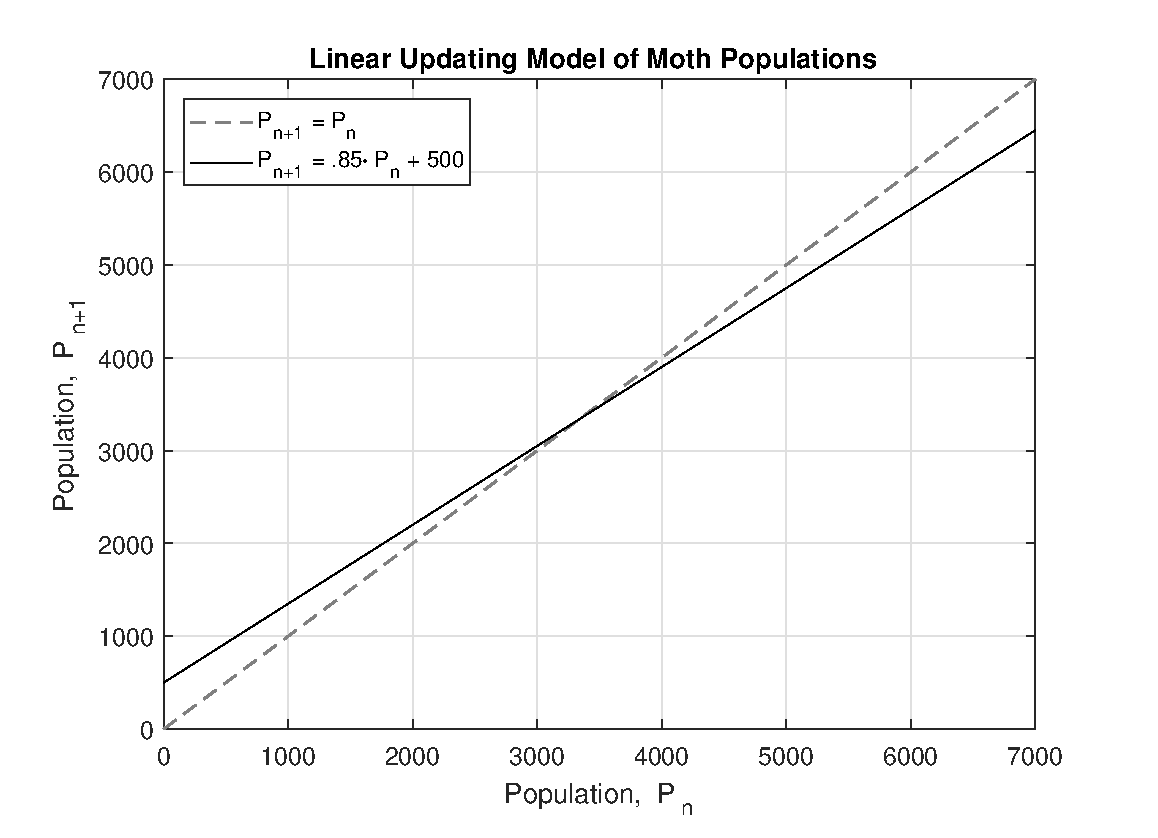
\includegraphics[width=12cm]{problem2.eps}}
	\caption{$P_{n+1}$ vs. $P_n$}
\end{figure}

\vspace{5mm}



\section*{Problem 4: More Moth Populations}

A different species of moth is examined here, this time using Hassell's population model and a starting population of 50. Figure 4 shows the population predicted by such a model, with 10 iterations of change. We can see that this particular model shows a dramatic increase in population with a relatively low starting population. This implies that a small starting population results in a huge population increase, and once the population explodes it shrinks very quickly afterwards. This could be due to a variety of issues: seasonal resource availability, predator behavior, or migration patterns. It should be noted that this population does have an equilibrium around 530, however a projection of this model shows that the updating model of population falls into a period-4 oscillation and remains there after even 1,000 iterations. This behavior is logical, as both equilibrium points are unstable and repelling.

\vspace{5mm}

\begin{figure}[H]
	\centering{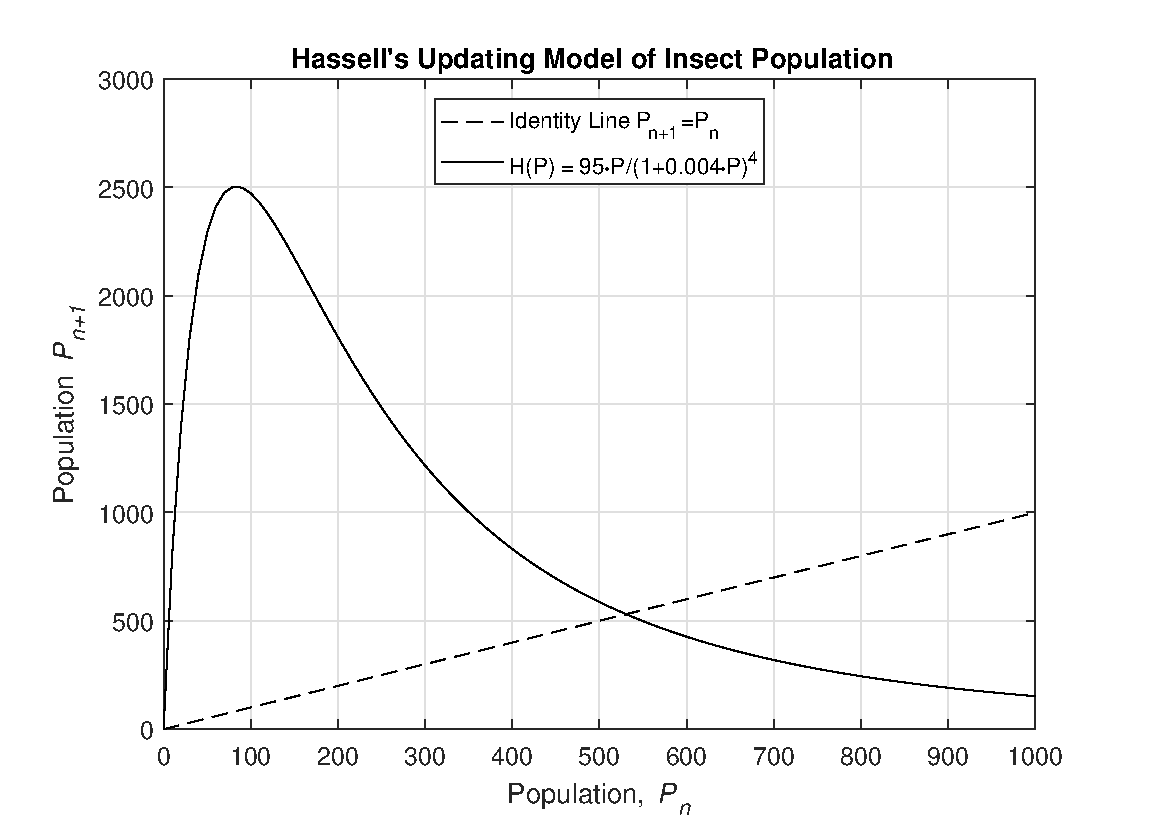
\includegraphics[width=12cm]{problem4.eps}}
	\caption{$P_{n+1}$ vs. $P_n$}
\end{figure}

\vspace{5mm}

\section*{Problem 5: Fishery Management}

There are many rules and regulation governing fishing practices in certain areas in order to prevent over-harvesting. Figure 5 presents a graph of a modified Ricker's model displaying two different harvesting intensity factors, {\it h}, with an initial population of 350. The top line represents a harvesting factor of .7, suggesting that this level of fishing will allow the population of fish to maintain an equilibrium at 500. The population briefly oscillates around this number before settling into a steady state. Conversely, a higher harvesting factor of 2.1 will dramatically reduce the population to below 100 before reaching an equilibrium at 200. 

The regulations surrounding fish harvesting are likely due to the need to keep populations above a certain level so that the ecology of their habitat remains stable. Adjusting the harvesting factor implies that regulations would be limited or expanded, allowing the population to remain at a desired number.

\vspace{5mm}

\begin{figure}[H]
	\centering{\includegraphics[width=12cm]{problem5.eps}}
	\caption{$P_{n+1}$ vs. $P_n$}
\end{figure}

\vspace{5mm}

\section*{Problem 6: Mexico and Population Models}

Like the Italy problem above, this one models Mexico's declining growth rate. Figure 6 shows us that Mexico has a negative-sloped linear growth rate as a best fit line to the data given between 1950 and 2000. The horizontal line represents the average growth rate, .287. The growth rate model fits the data reasonably well, although it appears that a better line might be fit if the 1950 growth rate were to be omitted. 

Figure 7 shows us how the population fits our linear growth rate along with a model that only accounts for a constant growth rate. We can see that a constant growth rate, given by the dashed line, may be unrealistic for future projections. The linear growth rate models the data much more accurately, and it is more realistic to expect a population to reach a maximum due to crowding effects. However, without much knowledge of the political and social situations governing birth and death rates in Mexico, it is hard to know how accurate either model might be. More research would yield a better analysis with a more dynamic growth rate model.

\vspace{5mm}

\begin{figure}[H]
	\centering{\includegraphics[width=12cm]{problem6.eps}}
	\caption{$k$ vs. $n$}
\end{figure}


\begin{figure}[H]
	\centering{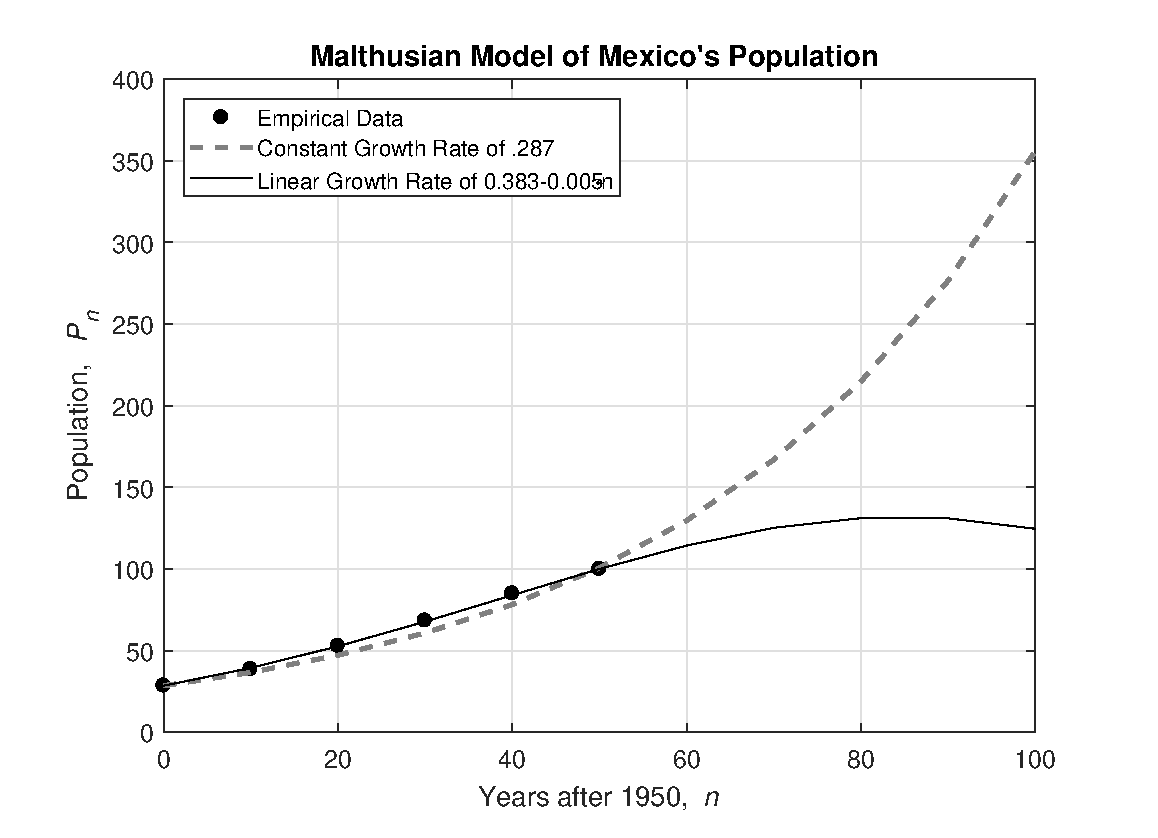
\includegraphics[width=12cm]{problem6b.eps}}
	\caption{$P$ vs. $n$}
\end{figure}

\vspace{5mm}

\section*{Problem 7: Saw-Tooth Grain Beetle and Population Models}

For this question the population of beetles was observed at 2-week increments for 30 weeks. Three models were used: The logistic model, the Beaverton-Holt model, and the Ricker's model. Each updating model is similar in that they predict a stable equilibrium at a population of $\approx $435 after about 20 weeks, as we can see with the intersection of the model with the identity line. We can see in Figure 8 that the three models appear quite similar, and that the beetle population does indeed level out at 435. The Beaverton-Holt looks like it hits the data points a bit more accurately, and indeed has a smaller sum of squared errors than the other two models.

Observing Figure 9 shows a more distinct difference between the models. These time series map the population growth up to 30 weeks. Clearly, the Beaverton-Holt model is the most accurate at predicting the population. This would be expected when comparing the sum of squared errors. Additionally, the percent errors for the Beaverton-Holt model are lower than the percent errors found in the other two models fairly consistently. While each model correctly predicts the carrying capacity of the population given the available resources, the Beaverton-Holt gives us a better picture of behavior before the equilibrium is reached. If the population were to sudden;y increase past the equilibria point, it is difficult to tell which model would be more accurate.

\vspace{5mm}

\begin{figure}[H]
	\centering{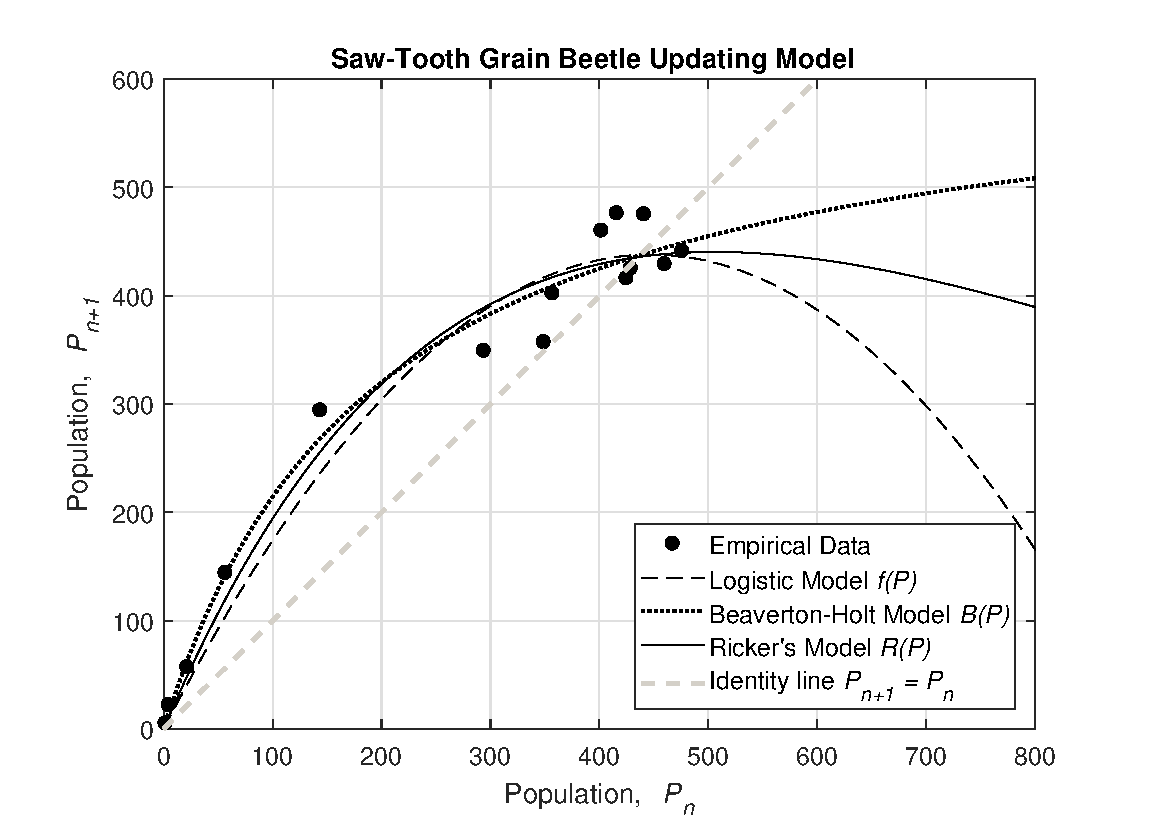
\includegraphics[width=12cm]{problem7a.eps}}
	\caption{$P_{n+1}$ vs. $P_n$}
\end{figure}

\vspace{5mm}



\vspace{5mm}

\begin{figure}[H]
	\centering{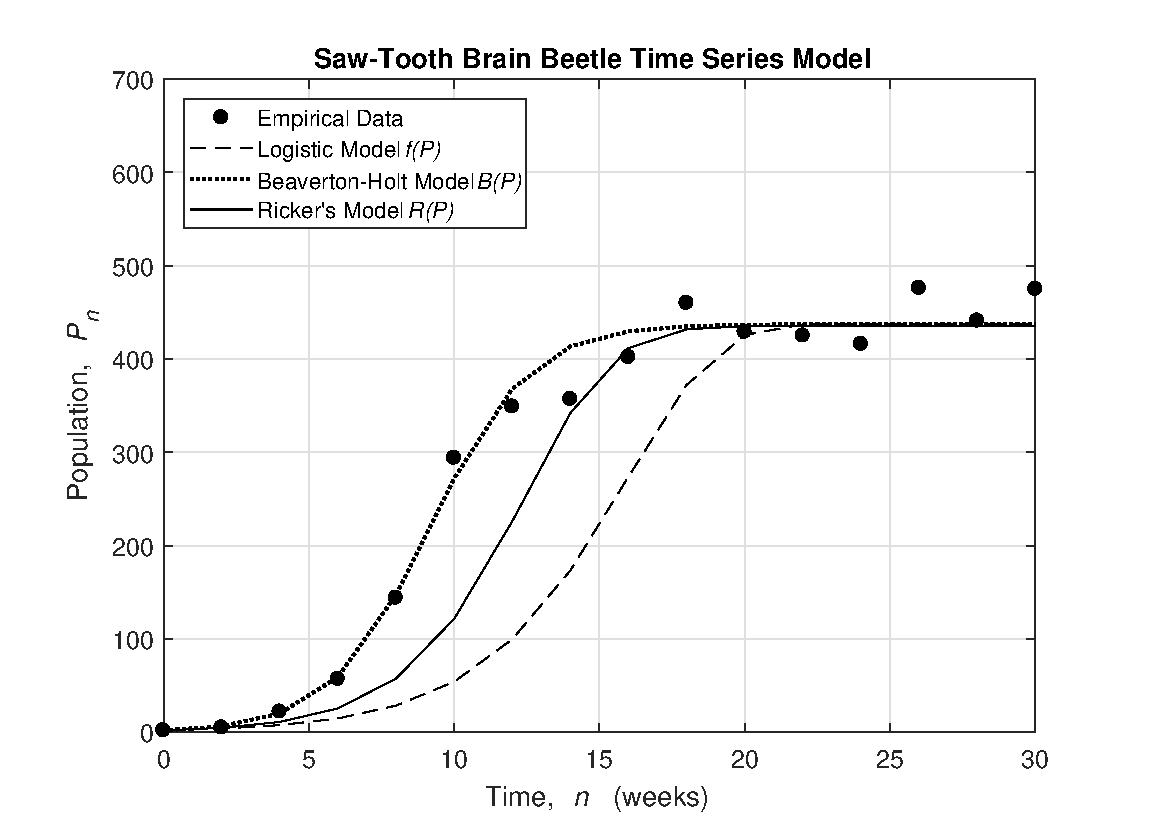
\includegraphics[width=11.75cm]{problem7b.eps}}
	\caption{$P_n$ vs. $n$}
\end{figure}

\vspace{5mm}



\section*{Problem 8: Bird Colony and Population Models}

Like the previous problem, we compare the efficacy of three models and observe their updating and time series representations. The updating models in Figure 10 show that the equilibrium is around 22 thousand, where the curves reach the identity line. The simple logistic growth model does not match the data as effectively as the other two models, and as expected, has a significantly higher sum of squared errors. The modified logistic growth model (adjusted for emigration) and the cubic growth model do not show a significant difference in this figure, however their difference is more pronounced in the time series model.

Figure 11 indeed highlights the differences among the models. The simple logistic model over-estimates the population, while the modified logistic model under-estimates the population. The cubic model is clearly more accurate, although it slightly over-estimates the population. We can also see that the cubic growth model oscillates around the equilibria, as indicated by the negative vale of that point when evaluated in the derivative. 

Other factors to consider include the stability of the equilibria and the percent error between the model and the data. While the cubic model is more accurate for early predictions, its equilibrium is unstable. This may result in highly inaccurate predictions for times greater than 10 years. The other two models have a stable equilibria, indicating that if the population is undisturbed, it will remain at a steady population. We can also observe that the cubic model has greater percent errors after 6 when compared to the percent errors of the other two models, likely due to the unstable oscillation mentioned previously.

\vspace{5mm}

\begin{figure}[H]
	\centering{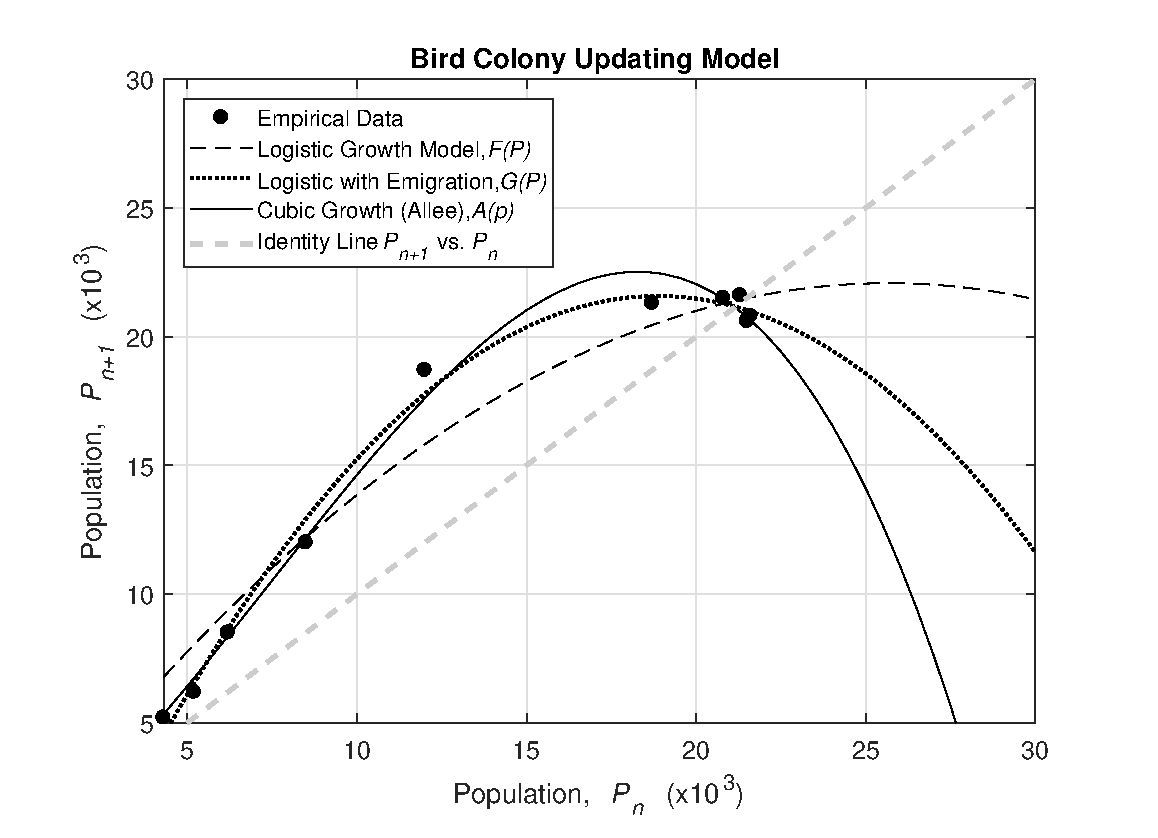
\includegraphics[width=12cm]{problem8a.eps}}
	\caption{$P_{n+1}$ vs. $P_n$}
\end{figure}

\begin{figure}[H]
	\centering{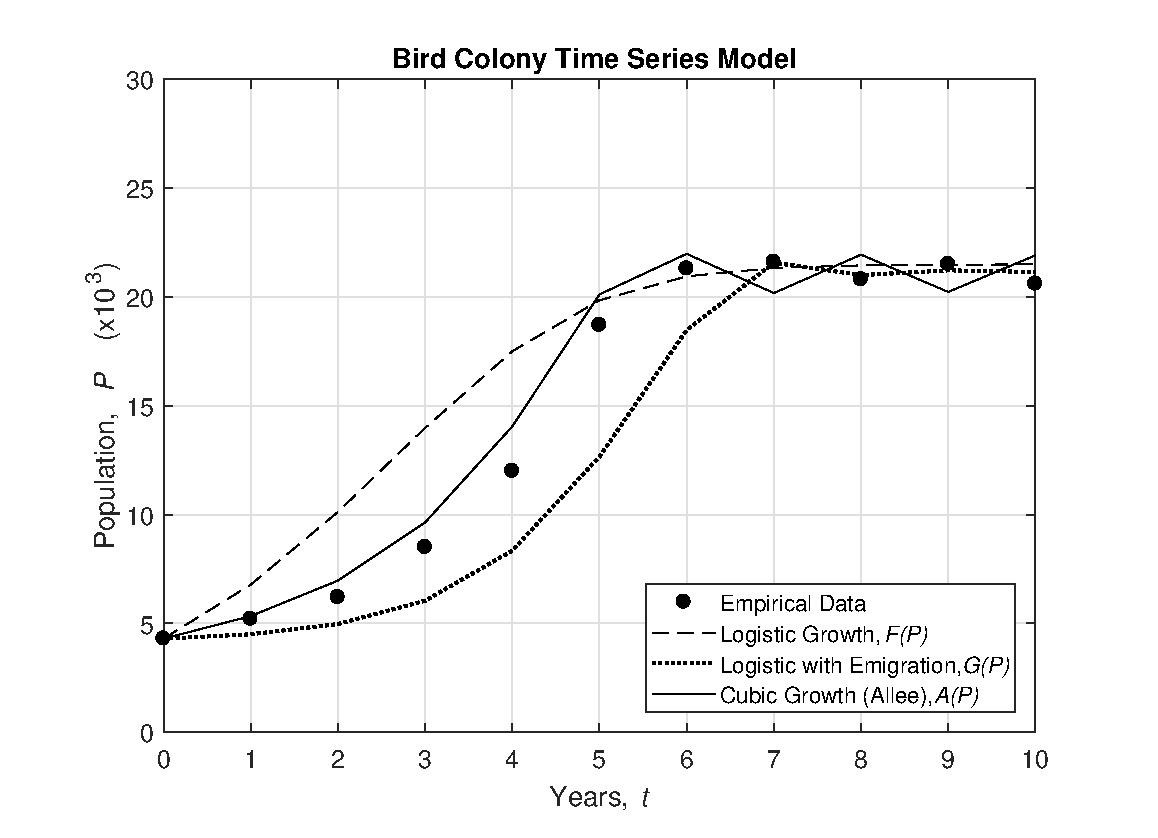
\includegraphics[width=12cm]{problem8b.eps}}
	\caption{$P$ vs. $t$}
\end{figure}

\vspace{5mm}



\section*{Model Analysis}

The Malthusian growth model modified for immigration is given by:

\vspace{5mm}

\begin{center}
	\begin{large}
	$P_{n+1}=(1+r)\cdot P_n+\mu$
	\end{large}
\end{center}

\vspace{5mm}

By continually composing this updating model with itself, we can determine populations in future iterations:

\begin{large}

\vspace{5mm}

$P_1=(1+r)\cdot P_0+\mu$

\vspace{2mm}

$P_2=(1+r)\cdot P_1+\mu \hspace{3mm} \longrightarrow \hspace{3mm} P_2=(1+r)^2\cdot P_0+(1+r)\cdot \mu+\mu$...

\vspace{2mm}

$P_4=(1+r)\cdot P_3+\mu \hspace{3mm} \longrightarrow \hspace{3mm} P_4=(1+r)^4\cdot P_0+(1+r)^3\cdot \mu+(1+r)^2\cdot \mu+(1+r)\cdot \mu+\mu$...

\vspace{2mm}

$P_n=(1+r)\cdot P_0+\mu\cdot\sum_{i=0}^{n-1}(1+r)^i$

\vspace{5mm}

\end{large}

We can also find the equilibria of this model by evaluating $P_{n+1}=P_n$ and solving for $P_n$. Doing this, we get $P_n=-\frac{\mu}{r}$. This tells us that $P$ will have a stable equilibria if $|\mu|<|r|$ and an unstable equilibria if $|\mu|>|r|$. If $|\mu|=|r|$ then we would need to investigate the particular function more deeply to determine the stability of the equilibrium point. We can also see that our equilibria will be monotonic if $\mu$ is negative and oscillatory of $\mu$ is positive. Translating this information to the model, we know that the model curve would cross the identity line at $-\frac{\mu}{r}$.

The Beaverton-Holt model is a bit more complex to analyze. It is given by:

\vspace{5mm}

\begin{large}

\begin{center}
	$P_{n+1}=\frac{a\cdot P_n}{1+b\cdot P_n}$
\end{center}

\end{large}

\vspace{5mm}

We can compare this to the previous model by using the Maclaurian series expansion to estimate the value of this function.

\begin{large}

\vspace{5mm}

$P_{n+1}\approx \frac{P_{n+1}(0)}{0!}\cdot P_n^0 + \frac{P_{n+1}'(0)}{1!}\cdot P_n^1 +\frac{P_{n+1}''(0)}{2!}\cdot P_n^2 +\frac{P_{n+1}'''(0)}{3!}\cdot P_n^3 +\frac{P_{n+1}''''(0)}{4!}\cdot P_n^4 +$...

\vspace{2mm}

$P_{n+1}\approx a\cdot P - a\cdot b\cdot P^2 + a\cdot b^2\cdot P^3 - a\cdot b^3\cdot P^4 +$...

\vspace{2mm}

$P_{n+1}\approx a\cdot \sum^{\infty}_{i=1} P_n^i\cdot b^{i-1}$

\vspace{5mm}

\end{large}

Here, the constant $a$ compares to $r$ because...



















Examining the equilibria of the Beaverton-Holt model, we find the usual stable point at $P_n=0$. The second equilibrium can be found when we factor out the $P_n$ from the equation $P_{n+1}-P_n=0$, and get $\frac {a}{1+b\cdot P_n}-1=0$. Solving for $P_n$, we see that it must be equal to $\frac{a-1}{b}$. To determine the stability, we must plug this value into the derivative $P'_{n+1}$: 

\begin{large}

\vspace{5mm}

$P'_{n+1}= \frac{a\cdot (1+b\cdot P_n)-a\cdot b\cdot P_n}{(1+b\cdot P_n)^2}$  $ \hspace{3mm}\longrightarrow \hspace{3mm}$  $P'_{n+1}(\frac{a-1}{b})= \frac{1}{a}$

\vspace{5mm}

\end{large}

In order to have a stable equilibria, $|a|\geq1$. Note that if $a=1$, we would only have one equilibrium point at $P_n=0$. Also, if $a$ is negative the model would show us oscillation at the equilibrium and if $a$ is positive we would see a monotonic increase to the equilibrium. 

To find an explicit solution for $P_n$, we can start by applying the transformation $P_n=\frac{1}{Y_n}$ so that $Y_{n+1}=\frac{1}{a}\cdot(Y_n+b)$. We can then use composition:

\begin{large}

\vspace{5mm}

$Y_1=\frac{1}{a}(Y_0+b)$

\vspace{2mm}

$Y_2=\frac{1}{a}(Y_1+b) \hspace{5mm} \longrightarrow \hspace{5mm} Y_2=\frac{1}{a^2}\cdot Y_0+\frac{1}{a}\cdot b+b$...

\vspace{2mm}

$Yn=\frac{1}{a^n}\cdot Y_0 + b\cdot \sum\frac{n-1}{i=1} \frac{1}{a^i}$

\vspace{5mm}

\end{large}

Therefore, our explicit solution to $P_{n+1}$ would look like:

 \vspace{5mm}
 
 \begin{large}
 	
 	$P_n=$ \begin{LARGE} $\frac{1}{a^{-n}\cdot P_0^{-1}+b\cdot \sum_{i=1}^{n-1}(\frac{1}{a})^i} $\end{LARGE}
 	
 \end{large}

\vspace{5mm}

Which would be a simple task for Matlab, yet gives many opportunities for mistakes when calculated by hand.


\end{document}





































